\documentclass[10pt]{article}
\usepackage{icmlko}

\icmlmeta{IP 파운데이션 월드모델}{335}{열 한 칸의 값}{축이 나빠서가 아니었다 --- 값을 섞은 위약이 똑같이 나쁘다}

\begin{document}

\twocolumn[
\icmlheader

\begin{abstract}
노트 334가 ``그림자를 다 지웠는데 축 둘을 되살리면 $-$0.0708(1/12)''로
끝내고 갈래 셋을 남겼다 --- ① 새로 긁은 자료가 거칠다 ② 열이 유보 25행에
많다 ③ 축이 원래 약했다. \textbf{셋을 다 쟀다.}

\textbf{① 반증.} 새로 긁은 68행이 오히려 깨끗하다 --- 매칭 후보가 하나뿐인
비율이 \textbf{49\% 대 21\%}, 관측률 84\% 대 80\%. 그리고 축$\sim$라벨
상관이 \emph{더} 세다(\texttt{goods\_scale} $+$0.490 대 $+$0.338).

\textbf{③ 반쯤 맞다 --- 그런데 방향이 거꾸로다.} 채택 검사로 보면 둘이
다르다: \texttt{goods\_scale} 은 검사 ①($\rho{=}{+}0.475$ · $p{<}$1e-4)과
②(시간 조각 \textbf{5/5})를 통과하고, \texttt{entry\_friction} 은
①($p{=}0.137$)도 ②(3/5, 최근 조각에서 부호가 뒤집힌다)도 떨어진다.
\textbf{그래서 굿즈만 되살리면 나을 것이라 미리 적었다.} 틀렸다 ---
굿즈만 $-$0.0506(2/12) · 정가만 $-$0.0644(2/12) · 둘 다 $-$0.0708(1/12)로
\textbf{셋이 다 비슷하게 나쁘다.}

\textbf{② 이것이 답이다.} \texttt{goods\_scale} 의 \emph{값만 섞은} 위약을
돌렸다 --- 열 수도 관측 무늬도 그대로고 정보만 없앤다(값$\sim$라벨
$+$0.542 $\to$ $-$0.009). \textbf{위약이 $-$0.0575(1/12)다.} 진짜가
$-$0.0456(2/12)이고 \textbf{진짜 $-$ 위약이 $+$0.0119(SD 0.0621 · 7/12)로
못 가른다.}

\textbf{손해는 열 그 자체다.} 유보 25행 · 학습 147행에서 관측된 열을 하나
더 붙이면 무엇이 들었든 약 $-$0.05 다. \textbf{그래서 채택 검사가 못 짚었다}
--- 검사는 축이 \emph{무엇을 아는가}를 재는데 비용은 축이 \emph{무엇을
아는가와 무관}하다.
\end{abstract}
]

\section{갈래 셋을 다 쟀다}

\begin{center}\footnotesize
\begin{tabular}{lll}
\hline
갈래 & 예측 & 결과 \\
\hline
① 새 자료가 거칠다 & 새 68이 나쁘다 & \textbf{반증}(더 깨끗) \\
③ 축이 원래 약하다 & 굿즈는 낫다 & \textbf{반증}(같다) \\
\textbf{② 열이 많다} & --- & \textbf{맞다} \\
\hline
\end{tabular}
\end{center}

\begin{figure*}[t]
\centering
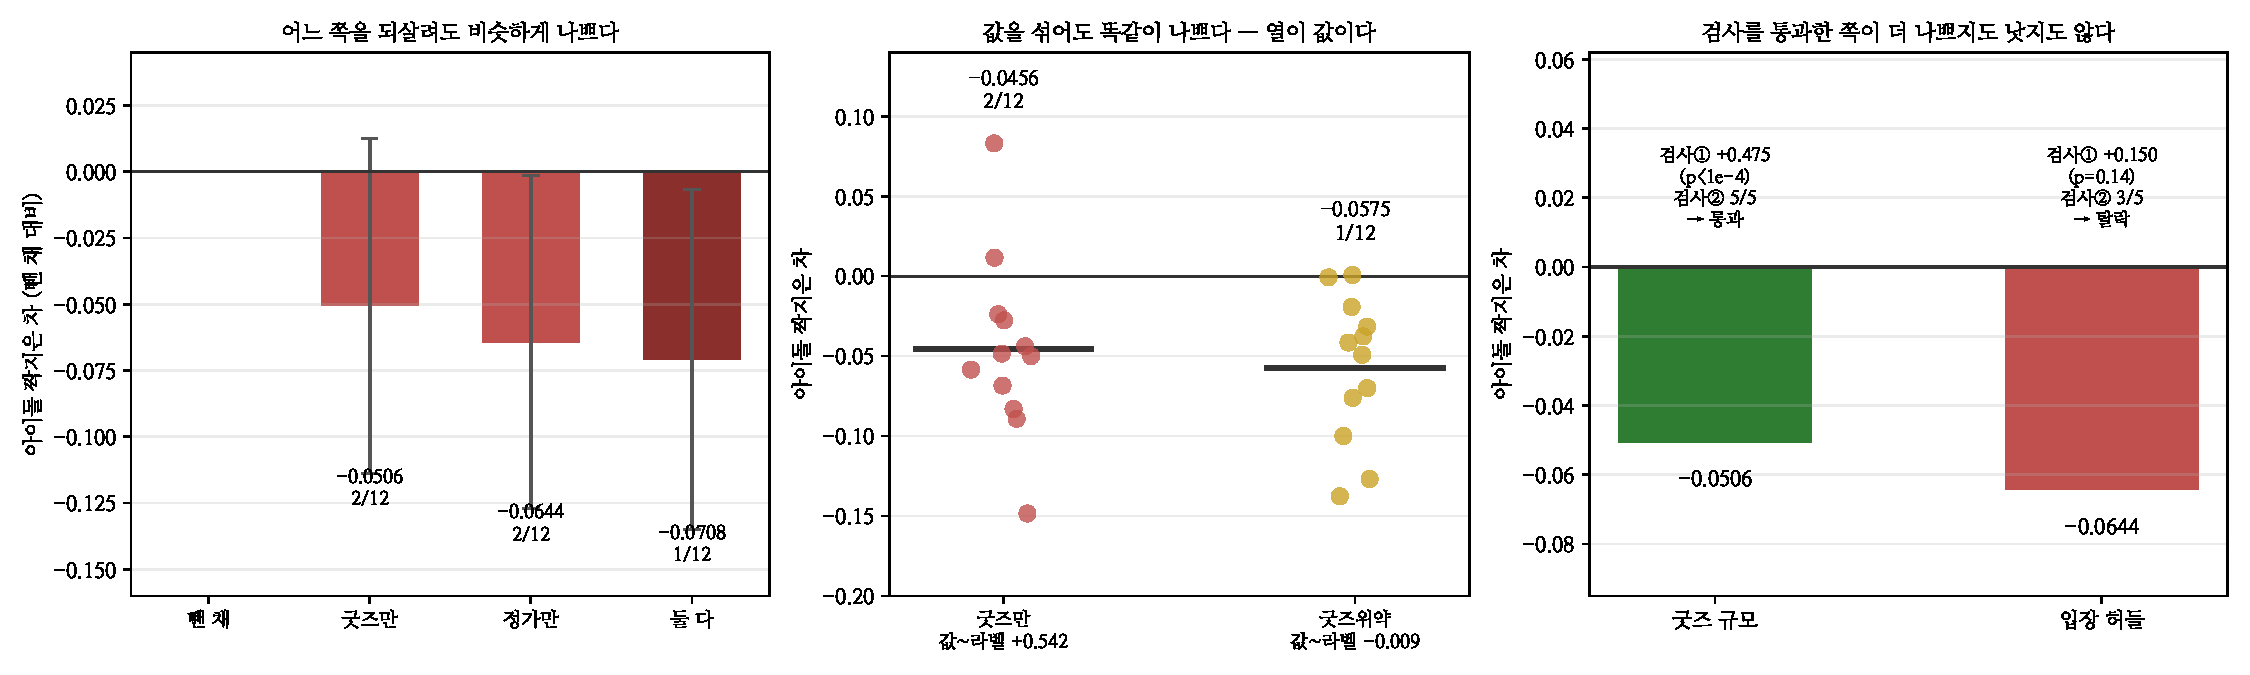
\includegraphics[width=\textwidth]{figs/column.pdf}
\caption{왼쪽 --- 축을 하나씩 되살릴 때. 가운데 --- 진짜 값과 섞은 값.
오른쪽 --- 채택 검사의 판정과 실제 값.}
\end{figure*}

\section{새로 긁은 것이 더 깨끗하다}

\begin{center}\footnotesize
\begin{tabular}{lrr}
\hline
 & 옛 79 & 새 68 \\
\hline
관측률(버전 · 정가) & 0.80 & \textbf{0.84} \\
매칭 후보 1건뿐 & 21\% & \textbf{49\%} \\
\texttt{goods\_scale}$\sim$라벨 & $+$0.338 & \textbf{$+$0.490} \\
\texttt{entry\_friction}$\sim$라벨 & $+$0.152 & \textbf{$+$0.288} \\
\hline
\end{tabular}
\end{center}

\textbf{덜 유명한 그룹이라 페이지가 거칠 것}이라는 짐작이 틀렸다. 오히려
후보가 적어 애매함이 덜하다.

\section{검사는 갈랐는데 판은 안 갈렸다}

\begin{center}\footnotesize
\begin{tabular}{lccr}
\hline
축 & 검사① & 검사② & 짝지은 차 \\
\hline
\texttt{goods\_scale} & \textbf{통과} & \textbf{5/5} & $-$0.0506 (2/12) \\
\texttt{entry\_friction} & 탈락 & 3/5 & $-$0.0644 (2/12) \\
둘 다 & --- & --- & $-$0.0708 (1/12) \\
\hline
\end{tabular}
\end{center}

노트 324가 ``검사는 거르지 줄 세우지 못한다''를 남겼다. \textbf{여기서는
더 나아간다} --- 검사를 통과한 축과 떨어진 축이 \emph{같은 값}을 갖는다.

\section{값을 섞어도 똑같다}

\texttt{goods\_scale} 의 관측된 값들만 무작위로 섞었다. 열 수 · 관측 무늬 ·
결측 자리가 전부 그대로고 \textbf{정보만 없다.}

\begin{center}\footnotesize
\begin{tabular}{lrrr}
\hline
 & 값$\sim$라벨 & 짝지은 차 & 양수 \\
\hline
굿즈만(진짜) & $+$0.542 & $-$0.0456 & 2/12 \\
\textbf{굿즈위약(섞음)} & \textbf{$-$0.009} & \textbf{$-$0.0575} & \textbf{1/12} \\
\hline
진짜 $-$ 위약 & & $+$0.0119 & 7/12 \\
\hline
\end{tabular}
\end{center}

\textbf{정보가 0 인 열이 정보가 있는 열만큼 나쁘다.} 그리고 둘의 차가
$+$0.0119(SD 0.0621)로 \textbf{0 과 못 가른다} --- 이 자리에서
\texttt{goods\_scale} 의 정보 값어치는 잴 수 없을 만큼 작다.

\section{그러면 비용이 어디서 오나}

\texttt{forms.\_design} 은 축마다 \textbf{값과 관측 표시자 두 열}을 싣는다.
아이돌은 유보 25행 · 학습 147행이고 이미 축 스물셋이다. 열 둘을 더하면
배깅부스트가 그만큼 더 갈 곳이 생기고, \textbf{25행으로는 그 갈림이 옳은지
확인할 수 없다.} 노트 331이 아이돌 흔들림의 72\%가 자료라 했던 것과 같은
자리다 --- \textbf{행이 모자란 곳에서는 열이 부채다.}

\begin{center}\small
\begin{tabular}{ll}
\hline
행을 더하면(노트 332 · 333) & 아이돌 \textbf{$+$0.25} \\
열을 더하면(오늘) & 아이돌 \textbf{$-$0.05} \\
\hline
\end{tabular}
\end{center}

\section{남은 것}
\begin{center}\footnotesize
\begin{tabular}{ll}
\hline
갈래 & 왜 \\
\hline
\textbf{다른 도메인의 열 비용} & 웹툰 711행에서도 $-$0.05 인가 \\
표시자 열을 빼면 & 값 열만 실으면 반값인가 \\
\textbf{노트 309 · 321 · 324 재해석} & ``축을 더했는데 안 올랐다'' \\
축 수를 줄이면 오르나 & 스물셋에서 열다섯으로 \\
\hline
\end{tabular}
\end{center}

\paragraph{규약} \textbf{축을 더하는 데는 정보와 무관한 값이 있다.}
이 실험실은 축 채택 검사 넷을 만들어 ``이 축이 무엇을 아는가''를 재 왔다
(노트 239 · 285 · 299 · 321). 오늘 잰 것은 그 반대편이다 --- \textbf{아무것도
모르는 열도 자리를 차지하고, 작은 도메인에서는 그 자리값이 축이 아는
것보다 크다.} 그래서 앞으로 축을 붙일 때는 검사 넷과 함께
\textbf{``이 도메인의 유보가 몇 행인가''}를 같이 적어야 한다. 그리고
\textbf{위약 열은 싸다} --- 값만 섞으면 되고, 한 번 돌리면 ``이 축이 버는가''를
``열이 드는가''와 갈라 준다.

\end{document}
